\chapter{Isolas of localized structures and Raman–Kerr frequency combs in micro-structured resonators (Chaos, Solitons \& Fractals 174, 113808)}

In section~\ref{sec:fra_LS} the concept of dissipative 
localized structures (LSs) was introduced. These states can be observed in a huge variety
of systems including vegetation patterns, biology, magnetic systems, fluids,
granular matter and nonlinear 
optics~\cite{tlidi2014localized,heimburg2005soliton,descalzi2011localized,purwins2010dissipative,ankiewicz2008dissipative,knobloch2015spatial}. 
In the case of nonlinear optical systems,
a particularly interesting type of localized structure can be identified,
the so-called optical solitons. Moreover, it has recently been discovered that the formation of solitons
in both fiber and micro-resonators gives rise to frequency combs, which are equally
spaced spectral lines. These frequency combs are exceedingly useful
for technological purposes such as chip-scale atomic clocks \cite{Jost2015clock}, terabit
per second communication \cite{marin2017microresonator} and even the calibration of spectrometers
for exoplanet search \cite{suh2019searching}. From a theoretical perspective, the dynamics
of solitons in these optical resonator systems can be accurately described 
by the forced dissipative nonlinear Schrödinger
equation~\cite{morales1974ponderomotive,nozaki1984solitons,kaup1978theory,ferre2017localized},
more commonly known as the Lugiato-Lefever equation\cite{lugiatolefever1987} in the context
of optical systems.

The aim of this chapter is the study of the formation of such structures in the
case of short solitons where the influence of the stimulated Raman scattering (SRS)
cannot be neglected and higher-order dispersion terms appear. In this case, a reduced model
in the form of a non-local Swift-Hohenberg equation is proposed to provide 
analytical results and an in-depth numerical description. By means of a combination of
numerical simulations and
continuation of the reduced model (see \ref{sec:cont_traveling} for a detailed discussion on the
continuation of traveling states), it can be seen that the SRS induces a forced symmetry
breaking leading to the motion of both the bright and dark solitons, as well as a disconnection between 
the different branches of LSs. Consequently, the traditional homoclinic snaking bifurcation diagram breaks
apart and instead, a family of isolas emerges. Lastly, a numerical analysis of the
original model, the generalized LLE, confirms both the formation of drifting LSs and
the presence of isolas due to the reflection symmetry breaking, in agreement with previous studies \cite{burke2009swift,parra2014third}.

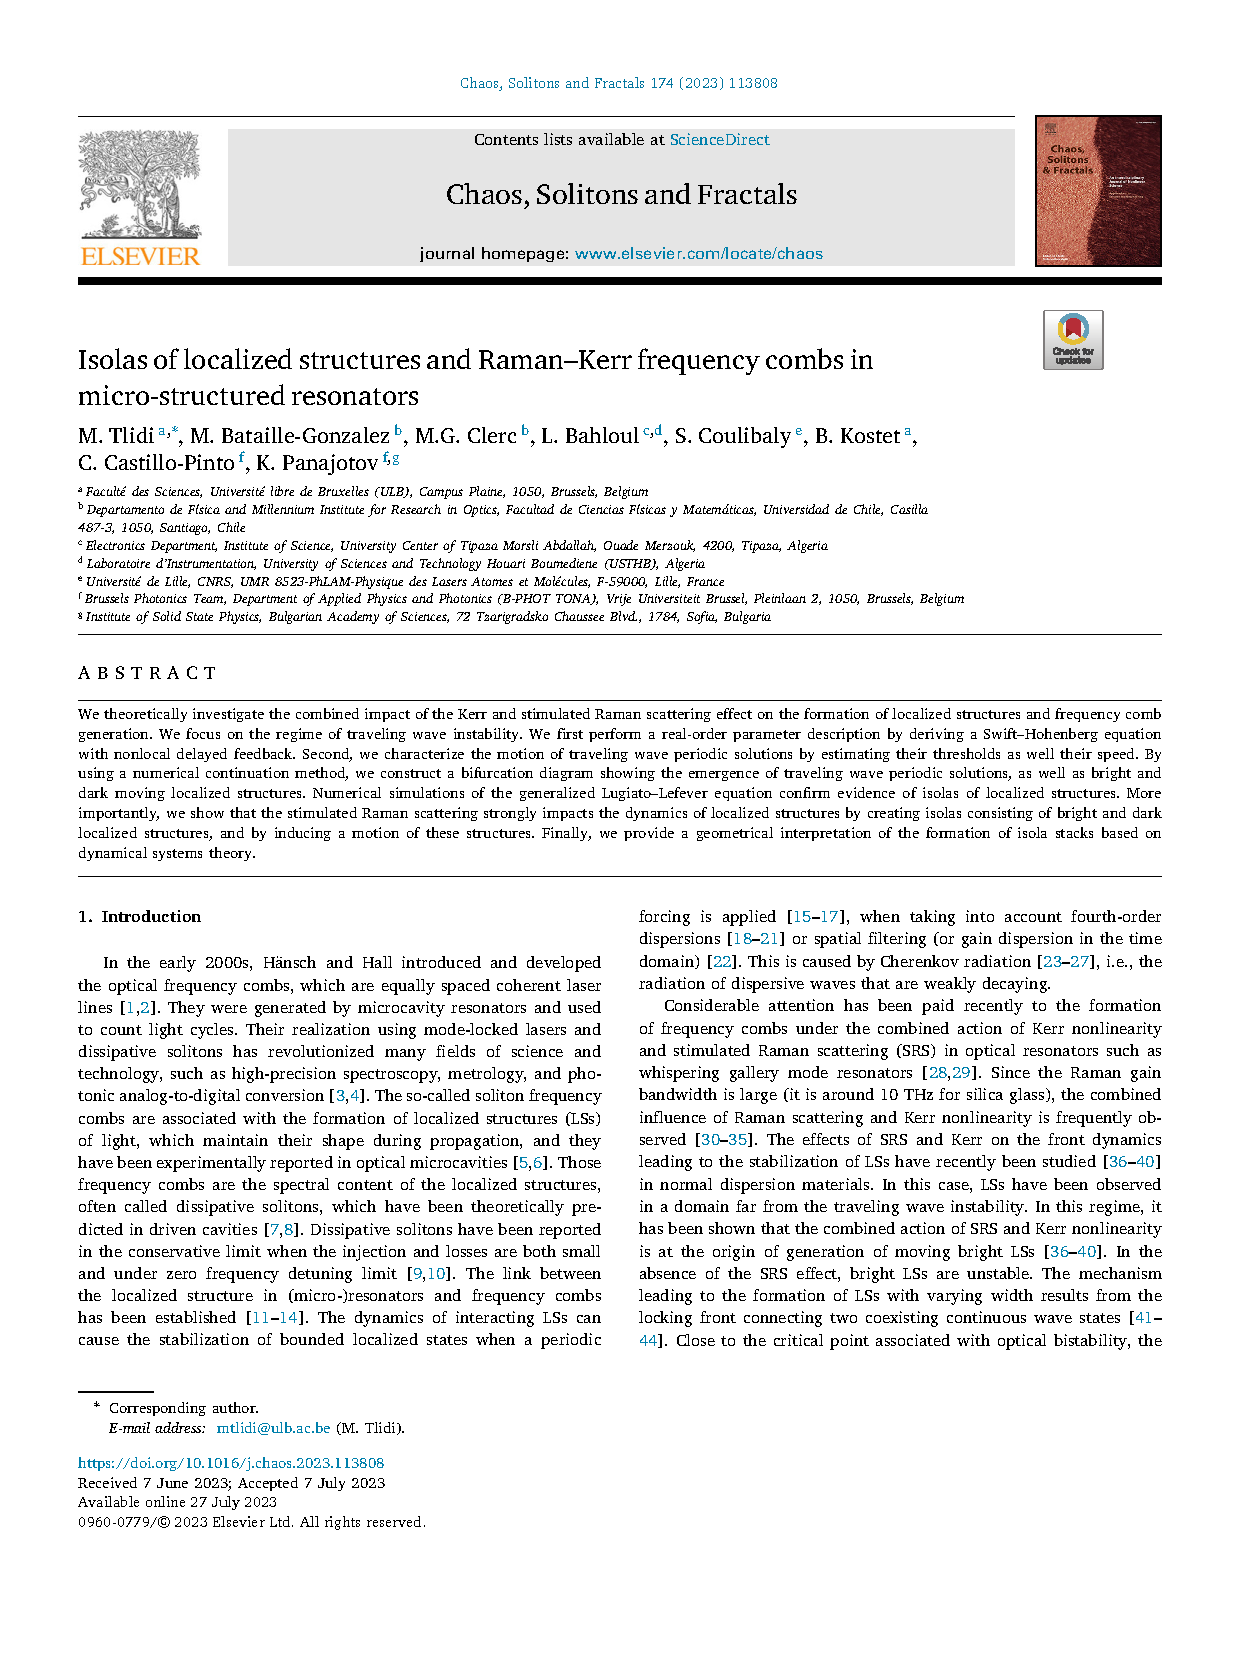
\includepdf[pages={-}]{chapters/isolas.pdf}

\section{Perspectives}

In this work, we have performed a detailed numerical analysis of the formation
of bright and dark solitons in a reduced non-local Swift-Hohenberg equation. More specifically,
the effect of a reflection symmetry-breaking term was investigated: the Raman effect on 
the LSs. Additionally, these results have been represented in a 
detailed bifurcation diagram. 
Nevertheless, not all of the bifurcations
present in the diagram were completely characterized.
For instance, the traveling 
wave and most LSs lose stability before the saddle-node bifurcation at an unidentified
bifurcation point. Thus, further work is needed in this direction.
 On the other hand, although the main results have been successfully
confirmed on the original model, a more complete bifurcation diagram, showing the stability and all of the LSs, 
remains
to be produced.
